\documentclass[12pt]{article}
\usepackage{graphicx}
%\usepackage{showframe}
\usepackage{subcaption}
\usepackage{wrapfig}
\begin{document}
\graphicspath{d:/LATEX courses}
\begin{figure}[h]
\centering
\begin{subfigure}[b]{0.4\linewidth}
\includegraphics[width=1.1\linewidth]{luo yi starlight}
\caption{LUO YI}
\end{subfigure}
\begin{subfigure}[b]{0.4\linewidth}
\includegraphics[width=1.1\linewidth]{luo yi mlbb}
\caption{Another luo yi}
\end{subfigure}
\caption{The two types of luo yi design}
\label{fig:LUO YI} \vspace{2cm}\hline \\
\end{figure}

\newpage
\begin{figure}
\begin{wrapfigure}{r}{0.5\linewidth}
\centering
\vspace{7pt}
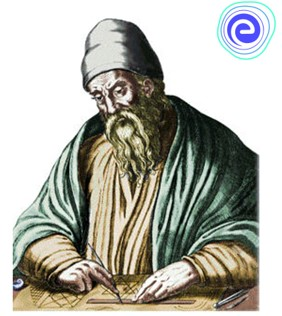
\includegraphics[width=1.1]{EUCLID 2}
\end{wrapfigure}
\textbf{A brief introduction of Euclid is provided below.}
\begin{itemize}
\item Euclid is one of the most prominent Greek\\mathematicians.\\
\item Little is known about his life, but there are\\only a handful of refrences to him.\\
\item A part from his words on geometry,in his\\book: Elements, nice results in Number the-\\ory can be noticed.
\end{itemize}
\end{figure}
\end{document}